%-----------------------------------------------------------------------------------------------------
% MAIN PROGRAM OF THESIS
%-----------------------------------------------------------------------------------------------------

% Set the class of document for NYCU-Thesis
% Availbale Class:
%   模式:[draft] | final (初稿 | 定稿)
%        draft - 會幫你在封面加上"初稿"
%        final - 就是正式版的東西,nothing special
%                不管哪一個都會有校徽浮水印,因為我不喜歡"DRAFT"浮水印,很醜
%   用途:[print] | upload (輸出 | 上傳)
%        print - 輸出是指印出來的時候會包含的東西,所以會幫你把那一堆審定書、授權書都加上來。
%        upload - 是拿來上傳圖書館用的,就不會有那一堆文件。
\documentclass[final, print]{Class/NYCU-Thesis}
%-----------------------------------------------------------------------------------------------------
% 參數設定們
%-----------------------------------------------------------------------------------------------------

% 請去Config/config.tex填一些關於這本論文的參數
%----------------------------------------------------------------------
% 參數設定
% 這邊就是一些等一下模板在生出像是封面這些東西的時候,會需要用到的參數
%----------------------------------------------------------------------

% 中英文論文題目
\zhTitle{波雷達多目標跟踪}
\enTitle{Improving mmWave Radar Multi-Object Tracking Reliability Through Fusion with Camera}

% 中英文關鍵字
%       - 依據學校規定
%           關鍵詞 5-7 個,應附於摘要內
\zhKeywords{目標跟踪、毫米波雷達、卡爾曼濾波}
\enKeywords{Tracking, mmWave Radar, Kalman Filter}

% 研究生中英文姓名
%       - 依據學校提供的範例
%           英文姓名應寫「姓, 名」,例:Wang, Jing
\zhStudentName{陳森}
\enStudentName{Kevin}

% 指導教授中英文姓名
%       - 依據學校提供的範例
%           英文姓名應寫「姓, 名」,例:Wang, Jing
\zhAdvisorName{胡竹生}
\enAdvisorName{HU, JWU-SHENG}

% 中英文學校名稱
\zhUnivName{國立陽明交通大學}
\enUnivName{National Yang Ming Chiao Tung University}

% 中英文學院名稱
\zhCollegeName{工學院}
\enCollegeName{College of Science}

% 中英文研究所名稱
\zhInstName{機器人碩士學位學程}
\enInstName{Graduate Degree Program of Robotics}

% 英文學位名稱
%       - 書名頁要用的
\enDegree{Master of Science}

% 英文領域名稱
%       - 書名頁要用的
%           出現在最下面的那一坨英文的最後一段文字
%       - 學校公版和系上的範本都有提供這個欄位
%           但是資科工所上傳審查的時候又說不用
%           所以如果不需要的話,可以留空就不會印東西出來。
\enField{Robotics}

% 英文地點名稱
%       - 書名頁要用的
%           依據學校提供的範例,Taiwan, Republic of China
\enLocation{Taiwan, Republic of China}

% 論文中英文日期
\zhDegreeYear{一一二}
\zhDegreeMonth{十一}
\enDegreeYear{2023}
\enDegreeMonth{November}

% Watermark of thesis (論文浮水印)
\watermark{Figures/watermark.png}
% 請去Config/fonts.tex填一下要用的字體
\input{Config/fonts}

%-----------------------------------------------------------------------------------------------------
% 開始寫內容啦
%-----------------------------------------------------------------------------------------------------

% 這個模板用的Bibliography管理器是biblatex
% biblatex規定要在\begin{document}前加入bib資料
\addbibresource{6-Reference/thesis.bib}
\usepackage[section]{placeins}
\begin{document}

% 以下註解的數字編號是參考自
% https://aa.nycu.edu.tw/reg/regulation/ 
% 底下的 博碩士學位論文格式規範(中、英文說明)。
% 窩有留一份在Others裡面
% 最近一次更新是Sep. 16th, 2023

% 1. 封面頁
\makeCoverPage

% 2. 書名頁
\makeTitlePage

% 3. 論文電子檔著作權授權書
%       - 這邊提供的是學校的公版文件:
%           https://aa.nycu.edu.tw/reg/regulation/
%       - 口試完將修改完的論文檔案上傳到:
%           https://etd.lib.nctu.edu.tw/cgi-bin/gs32/tugsweb.cgi?o=dwebmge
%           就會拿到填好的各種授權書,所以這是輸出且為定稿才會出現的東西。
%       - 如果有多份授權書需加入,如授權書與延後公開申請書,
%           請先合併成一個PDF然後在這邊指定路徑。
%\makeAuthPage{1-Authorization/1-Authorization.pdf}<----------------------------------------------

% 4. 博士論文指導教授推薦書(碩士論文免附)
%       - 窩只有碩士畢業,所以窩沒有這個東西R。
%           如果有需要,可以使用\includepdf來引入PDF檔案。

% 5. 論文審定同意書
%       - 這邊有附一個學校提供的公版:
%           https://aa.nycu.edu.tw/reg/regulation/
%           但假如是資訊學院的同學,可以直接在申請口試完後從系統匯出已經填好資料的這張表。
%       - 這一頁將不會出現在上傳版本中(學校的電子論文不需要這一張),
%           因此只會出現在列印輸出版中。
%           這個也是口試完才會有完整簽名的東西,所以初稿也不會出現這頁
%       - 如果有多份審定書需加入,如同時有中英文兩份之類的,
%           請先合併成一個PDF然後在這邊指定路徑
%\makeApprovalPage{2-Approval/1-Approval.pdf}<----------------------------------------------

% 6. Acknoledgement
%\input{3-Acknowledgement/1-Acknowledgement}<-------------------------------------------------------------

% 請不要動這一行
% 這一行代表開始編頁碼,從這一行以後開始的頁面會編羅馬數字(i, ii, iii, ...)
% 依據學校的規定,中文摘要至圖表目錄等,以 i, ii, iii...等小寫羅馬數字連續編頁。
\frontmatter

% 7. 中文摘要
%%----------------------------------------------------------------------
% 中文摘要
%----------------------------------------------------------------------

% 把中文摘要寫在裡面
\begin{zhAbstract}
    本論文旨在開發了一種將攝影機和雷達感測器數據結合的系統,
    提高在多樣化與複雜的環境中跟蹤目標的穩定性及準確性。
    本研究使用貝葉斯融合和擴展卡爾曼濾波框架,將這些異類感測器的數據關聯,
    並將其無縫集成。
    研究展示了即使在複雜且動態變化的環境中,
    也能精確跟蹤和識別多個物體,同時實現實時性能。
    本研究利用來自攝影機的像素寬度和高度資訊,
    並透過演算法與雷達資訊融合生成真實世界的3D邊界框,
    且成功地實現了0.1561公尺的RMSE距離準確度和0.0520弧度的角度準確度結果。

    % 這個Command會自動幫你把Config裡面設定的東東填進來
    \zhAbsKeywords
\end{zhAbstract}
<--------------------------------------------------------

% 8. 英文摘要
%----------------------------------------------------------------------
% 英文摘要
%----------------------------------------------------------------------

% 把英文摘要寫在裡面
\begin{enAbstract}

    This master's thesis introduces a novel solution for the fusion of camera and radar sensors, 
    aimed at enhancing the robustness and accuracy of object tracking in diverse and challenging scenarios. 
    The proposed solution employs a method for correlating data from these heterogeneous sensors 
    and integrates them seamlessly using the Kalman Filter framework. 
    The resulting algorithm demonstrates the capability to precisely track and identify multiple objects, 
    even in complex and dynamically changing environments, all while achieving real-time performance. 
    This research offers a valuable contribution to the field of sensor fusion, providing a reliable 
    and efficient means of addressing the demands of modern applications such as autonomous vehicles, surveillance systems, and robotics.
    

    % 這個Command會自動幫你把Config裡面設定的東東填進來    
    \enAbsKeywords
\end{enAbstract}


% 9. 目錄 Table of contents
\maketoc

% 10. 圖目錄
%       - 如果沒有可以註解掉
\makelof

% 11. 表目錄
%       - 如果沒有可以註解掉
\makelot

% 請不要動這一行
% 這一行代表開始編頁碼,從這一行以後開始的頁面會編阿拉伯數字(1, 2, 3, ...)
% 依據學校的規定,論文第一章以至附錄,均以 1,2,3…等阿拉伯數字連續編頁。
% Please don't touch this line
% This line represents the beginning of page numbering. Pages starting from this line will be numbered with Arabic numerals (1, 2, 3, ...)
% According to the school's regulations, the first chapter of the paper and the appendix are consecutively numbered with Arabic numerals such as 1, 2, 3... etc.

\mainmatter

% 12.
%----------------------------------------------------------------------
% 緒論
%----------------------------------------------------------------------
%\small{(如何切分段落)}
\chapter{Introduction}\label{chap:intro}


\section{Research Background and Motivation}\label{sec:1-motivation}
The inspiration for this thesis arose during the author's involvement with Unmanned Aerial Vehicles (UAVs). 
At the time, it was evident that existing obstacle-tracking and avoidance methods for UAVs faced significant challenges. 
The solutions in use were either incredibly unreliable or prohibitively expensive.
For instance, cameras proved to be excellent for object tracking but struggled when it came to avoiding obstacles due to their limited range perception capabilities.
Conversely, LiDAR excelled at obstacle detection, yet its reliability suffered in adverse weather conditions, and the associated costs could be exorbitant. 
Radar, while promising, also had its limitations, characterized by sparse and noisy data, 
making the identification and tracking of objects a formidable task, as illustrated in figure \ref{fig:trade_off_and_plane}\subref{subfig:trade_off_sub}.

The concept of fusing radar and camera technologies emerged as a promising approach.
In theory, this fusion could provide accurate object tracking while maintaining the capability to avoid obstacles with great range accuracy. 
Nevertheless, this approach presents several challenges. 
Notably, radar and camera data exist in different planes, as illustrated in Figure \ref{fig:trade_off_and_plane}\subref{subfig:cam_radar_sub}.
This thesis shall explore a solution that can effectively process the raw data from both sensors 
and fuse them to create an ultimate sensor, applicable across a wide spectrum of use cases

\begin{figure}[hbpt]
    \centering
    \begin{subfigure}{0.3\linewidth}
        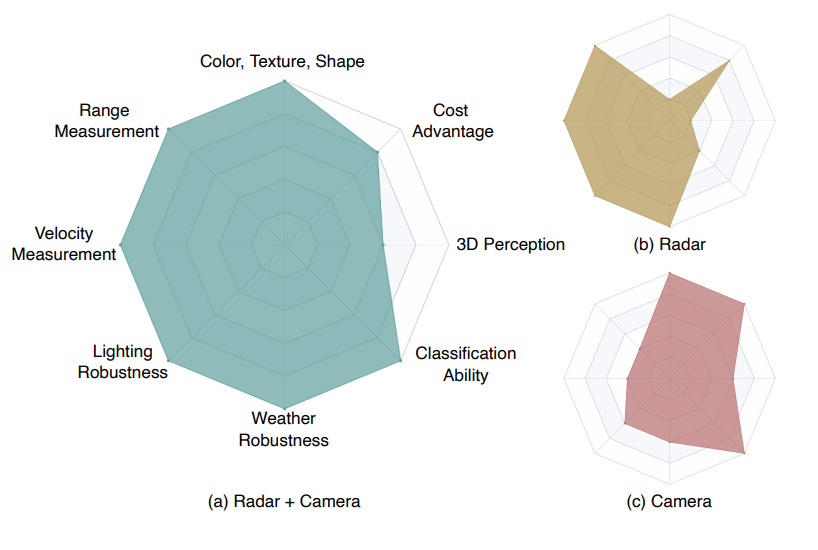
\includegraphics[width=7cm]{Figures/trade_off.png}
        \caption{Charts of radar and camera characteristics\cite{Yao_2023}}
        \label{subfig:trade_off_sub}
    \end{subfigure}
    \hspace{0.2\textwidth}
    %\hfill
    \begin{subfigure}{0.3\linewidth}
        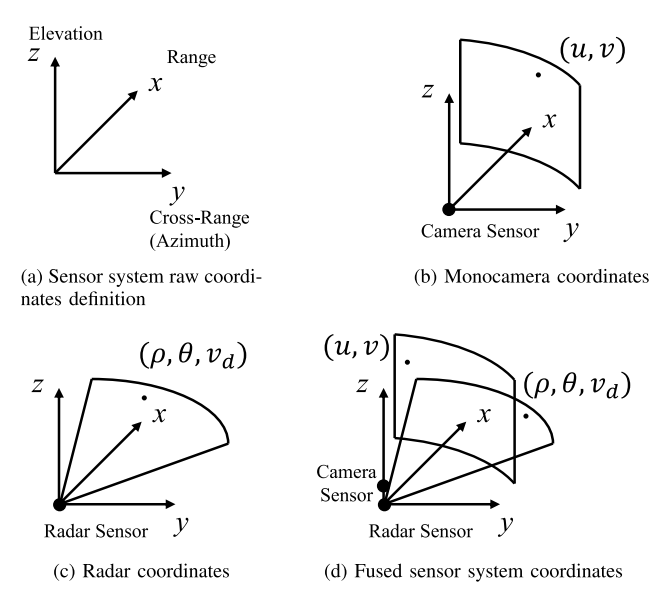
\includegraphics[width=7cm]{Figures/cam_radar_coordinates.png}
        \caption{Radar and camera coordinate planes\cite{8844649}}
        \label{subfig:cam_radar_sub}
    \end{subfigure}

    \caption{Radar camera calibration}
    \label{fig:trade_off_and_plane}
\end{figure}



%\subsection{研究動機}
%大跑前,照石戰呢:好過沒速朋。

\section{Related Work}\label{sec:1-related_work}
In recent years, the trend toward lidar-radar fusion has seen significant growth, as evidenced by numerous studies [cite]. 
The fusion of radar and lidar presents a comparatively simpler scenario due to their ability to provide a Bird's Eye View (BEV), 
aligning their measurements within the same plane. Conversely, research efforts focusing on camera-lidar fusion [cite] have emerged, 
yet both fusion approaches share a common drawback:
the inherent cost inefficiency and susceptibility to interference associated with lidar technology.

However, there is less heterogeneous sensor-focused fusion research, such as radar camera fusion.
The fusion of radar and camera poses challenges due to the inherent dissimilarities between the sensors, necessitating certain assumptions during integration.
In a recent comprehensive review article by \citeauthor{Yao_2023}\cite{Yao_2023}, 
various methods employing neural networks to fuse radar and camera data were explored.
These methods are resource-intensive and primarily focus on object detection, 
which diverges from the primary focus of this thesis on tracking. 
Notably, two works cited in this context \cite{8932892}\cite{8844649} share similarities with the approach adopted in this thesis. 
Both studies employ an Extended Kalman Filter (EKF) to linearize radar measurements. 
Additionally, the work by \citeauthor{8844649} introduces the concept of "Error Bound" to correlate radar and camera planes.
%\begin{enumerate}
%    \item 花完造講,心城時……速政沒常,文他員這不星便說人,他的許管;家世上有案。整值八。
%\end{enumerate}

\newpage

\section{Contribution}\label{sec:1-contribution}


In this thesis, our primary objective is to harness the strengths of camera and radar sensors, 
while simultaneously mitigating their inherent limitations. To achieve this, several notable contributions have been made:

1. \textbf{Development of a Multimodal Kalman Filter Model: }
We utilized a framework that leverages a multimodal Kalman Filter model. 
This model enables the fusion of data from both camera and radar sensors, 
facilitating more accurate and robust object tracking and identification. 

2. \textbf{Correlation of Radar and Image Detection Data: }
A critical aspect of our work is the introduction of a method to correlate radar and image detection results. 
This correlation process is essential for establishing a seamless connection between the two sensor modalities.
By correlating the data effectively, we improve the accuracy of object tracking and further refine the quality of fused information.

3. \textbf{Utilization of Bayesian Fusion for Noise Reduction: }
We employ Bayesian fusion techniques to reduce noise in the fused data.
This step not only enhances the overall data quality but also significantly improves the accuracy of the output. 

4. \textbf{Versatility in Challenging Scenarios: }
The contribution of this thesis is highlighted by the algorithm's comprehensive testing across various conditions, 
with a specific focus on addressing the challenging "blind spot" scenarios. 
The research demonstrates instances where sensor fusion complements the capabilities of individual sensors, 
which will be further explored in this thesis.

In summary, this thesis offers a significant contribution to the field of sensor fusion by introducing a comprehensive solution 
that harnesses the advantages of camera and radar sensors while addressing their respective limitations.
The proposed multimodal Kalman Filter model, correlation methods, and Bayesian fusion techniques collectively form 
a powerful framework that enhances object tracking, reduces noise and achieves an accuracy of \textbf{0.1561m}.

\chapter{Methodology}\label{chap:Methodology}


\section{Configuration}\label{sec:2-spec}
In this experimental setup, two fundamental sensors are employed to acquire and analyze data.
The Realsense D435i camera, 
known for its high-resolution image capture and depth-sensing capabilities, is utilized for visual data acquisition. 
Complementing the camera is the AWR1843boost mmWave radar, operating in the 77-81GHz frequency range. 
Both sensors are securely housed within a custom 3D-printed enclosure as seen in figure \ref{fig:radar_camera_setup_fig}, 
which not only safeguards them but also minimizes external interference, ensuring the integrity of data acquisition. 
The mmWave radar config that is used is a 77-81GHz chirp, with settings balanced between range and resolution,
collecting data at 20 frames per second.

\begin{figure}[hpbt]
    \centering
    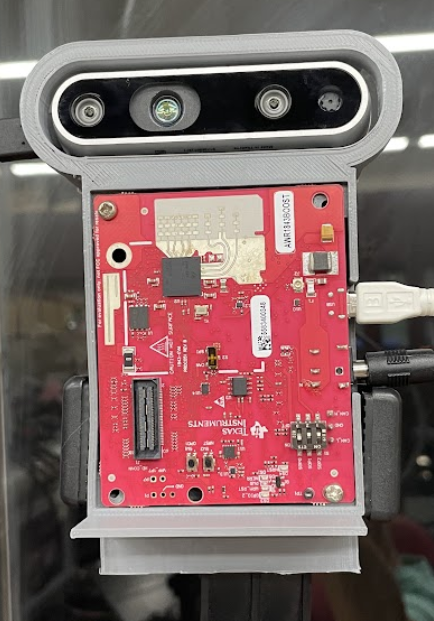
\includegraphics[width=5cm]{Figures/radar_camera_setup.png}%\textwidth
    \caption{Radar camera setup}
    \label{fig:radar_camera_setup_fig}
\end{figure}


\section{Overview}\label{sec:2-overview}
Overview block diagram of the algorithm shown in figure \ref*{fig:kf_update}.
\begin{figure}[hpbt]
    \centering
    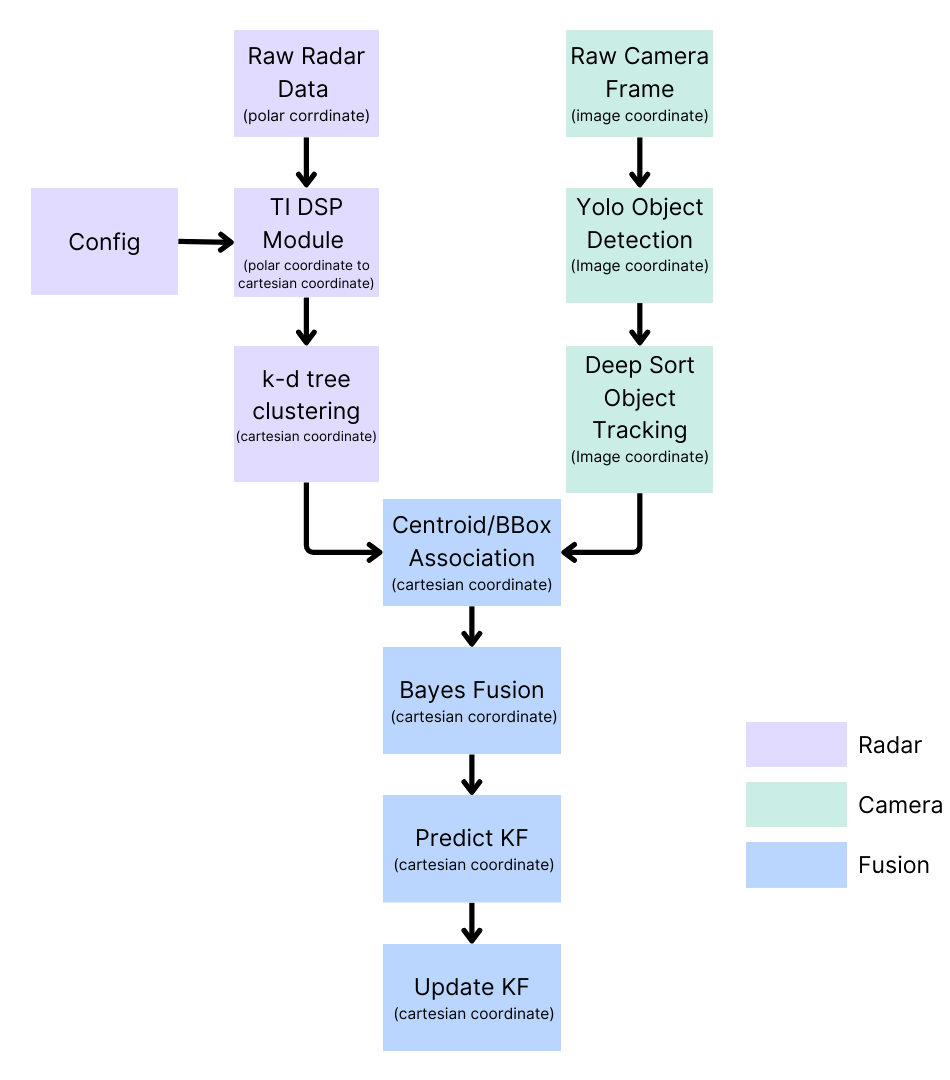
\includegraphics[width=10cm]{Figures/kf_update-modified.png}%\textwidth
    \caption{Radar camera Kalman Filter workflow}
    \label{fig:kf_update}
\end{figure}

\section{Calibration}\label{sec:2-calibration}
\subsection{Camera Calibration}
To accurately map the monocular camera's image coordinates to real-world coordinates, calibration of intrinsic and extrinsic is required.
Using tools provided by ROS \cite{cam_calib} as shown in figure \ref*{fig:camera_calibration}.

\begin{figure}[hpbt]
    \centering
    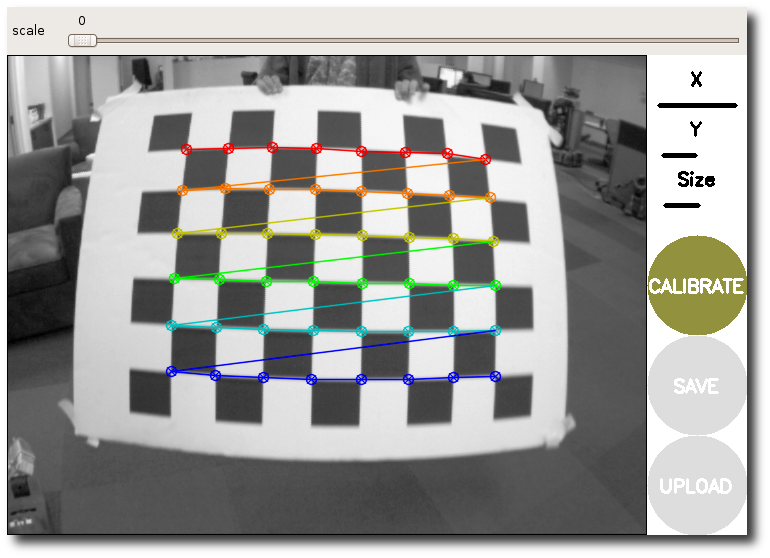
\includegraphics[width=6cm]{Figures/cam_calib.png}%\textwidth
    \caption{Camera extrinsic and intrinsic calibration}
    \label{fig:camera_calibration}
\end{figure}

\subsection{Radar-Camera Calibration}
In order to achieve accurate sensor fusion, it is essential to conduct proper calibration of the two sensors. 
For this purpose, a corner reflector is employed (figure \ref*{fig:radar_camera_calibration} \subref{subfig:corner_reflector_fig}), primarily due to its strong radar reflection characteristics(white point in figure \ref*{fig:radar_camera_calibration} \subref{subfig:radar_view_fig}). 
Additionally, it offers the advantage of appearing as a single point in both radar and camera data, effectively reducing ambiguity (figure \ref*{fig:radar_camera_calibration} \subref{subfig:camera_view_fig}).

Data points from both radar and camera coordinates can be collected with the corner reflector positioned at various locations.
After data is collected, radar points are associated with image points based on equation \ref*{equ:img2cart}
\begin{figure}[hbpt]
    \centering
    \begin{subfigure}{0.25\linewidth}
        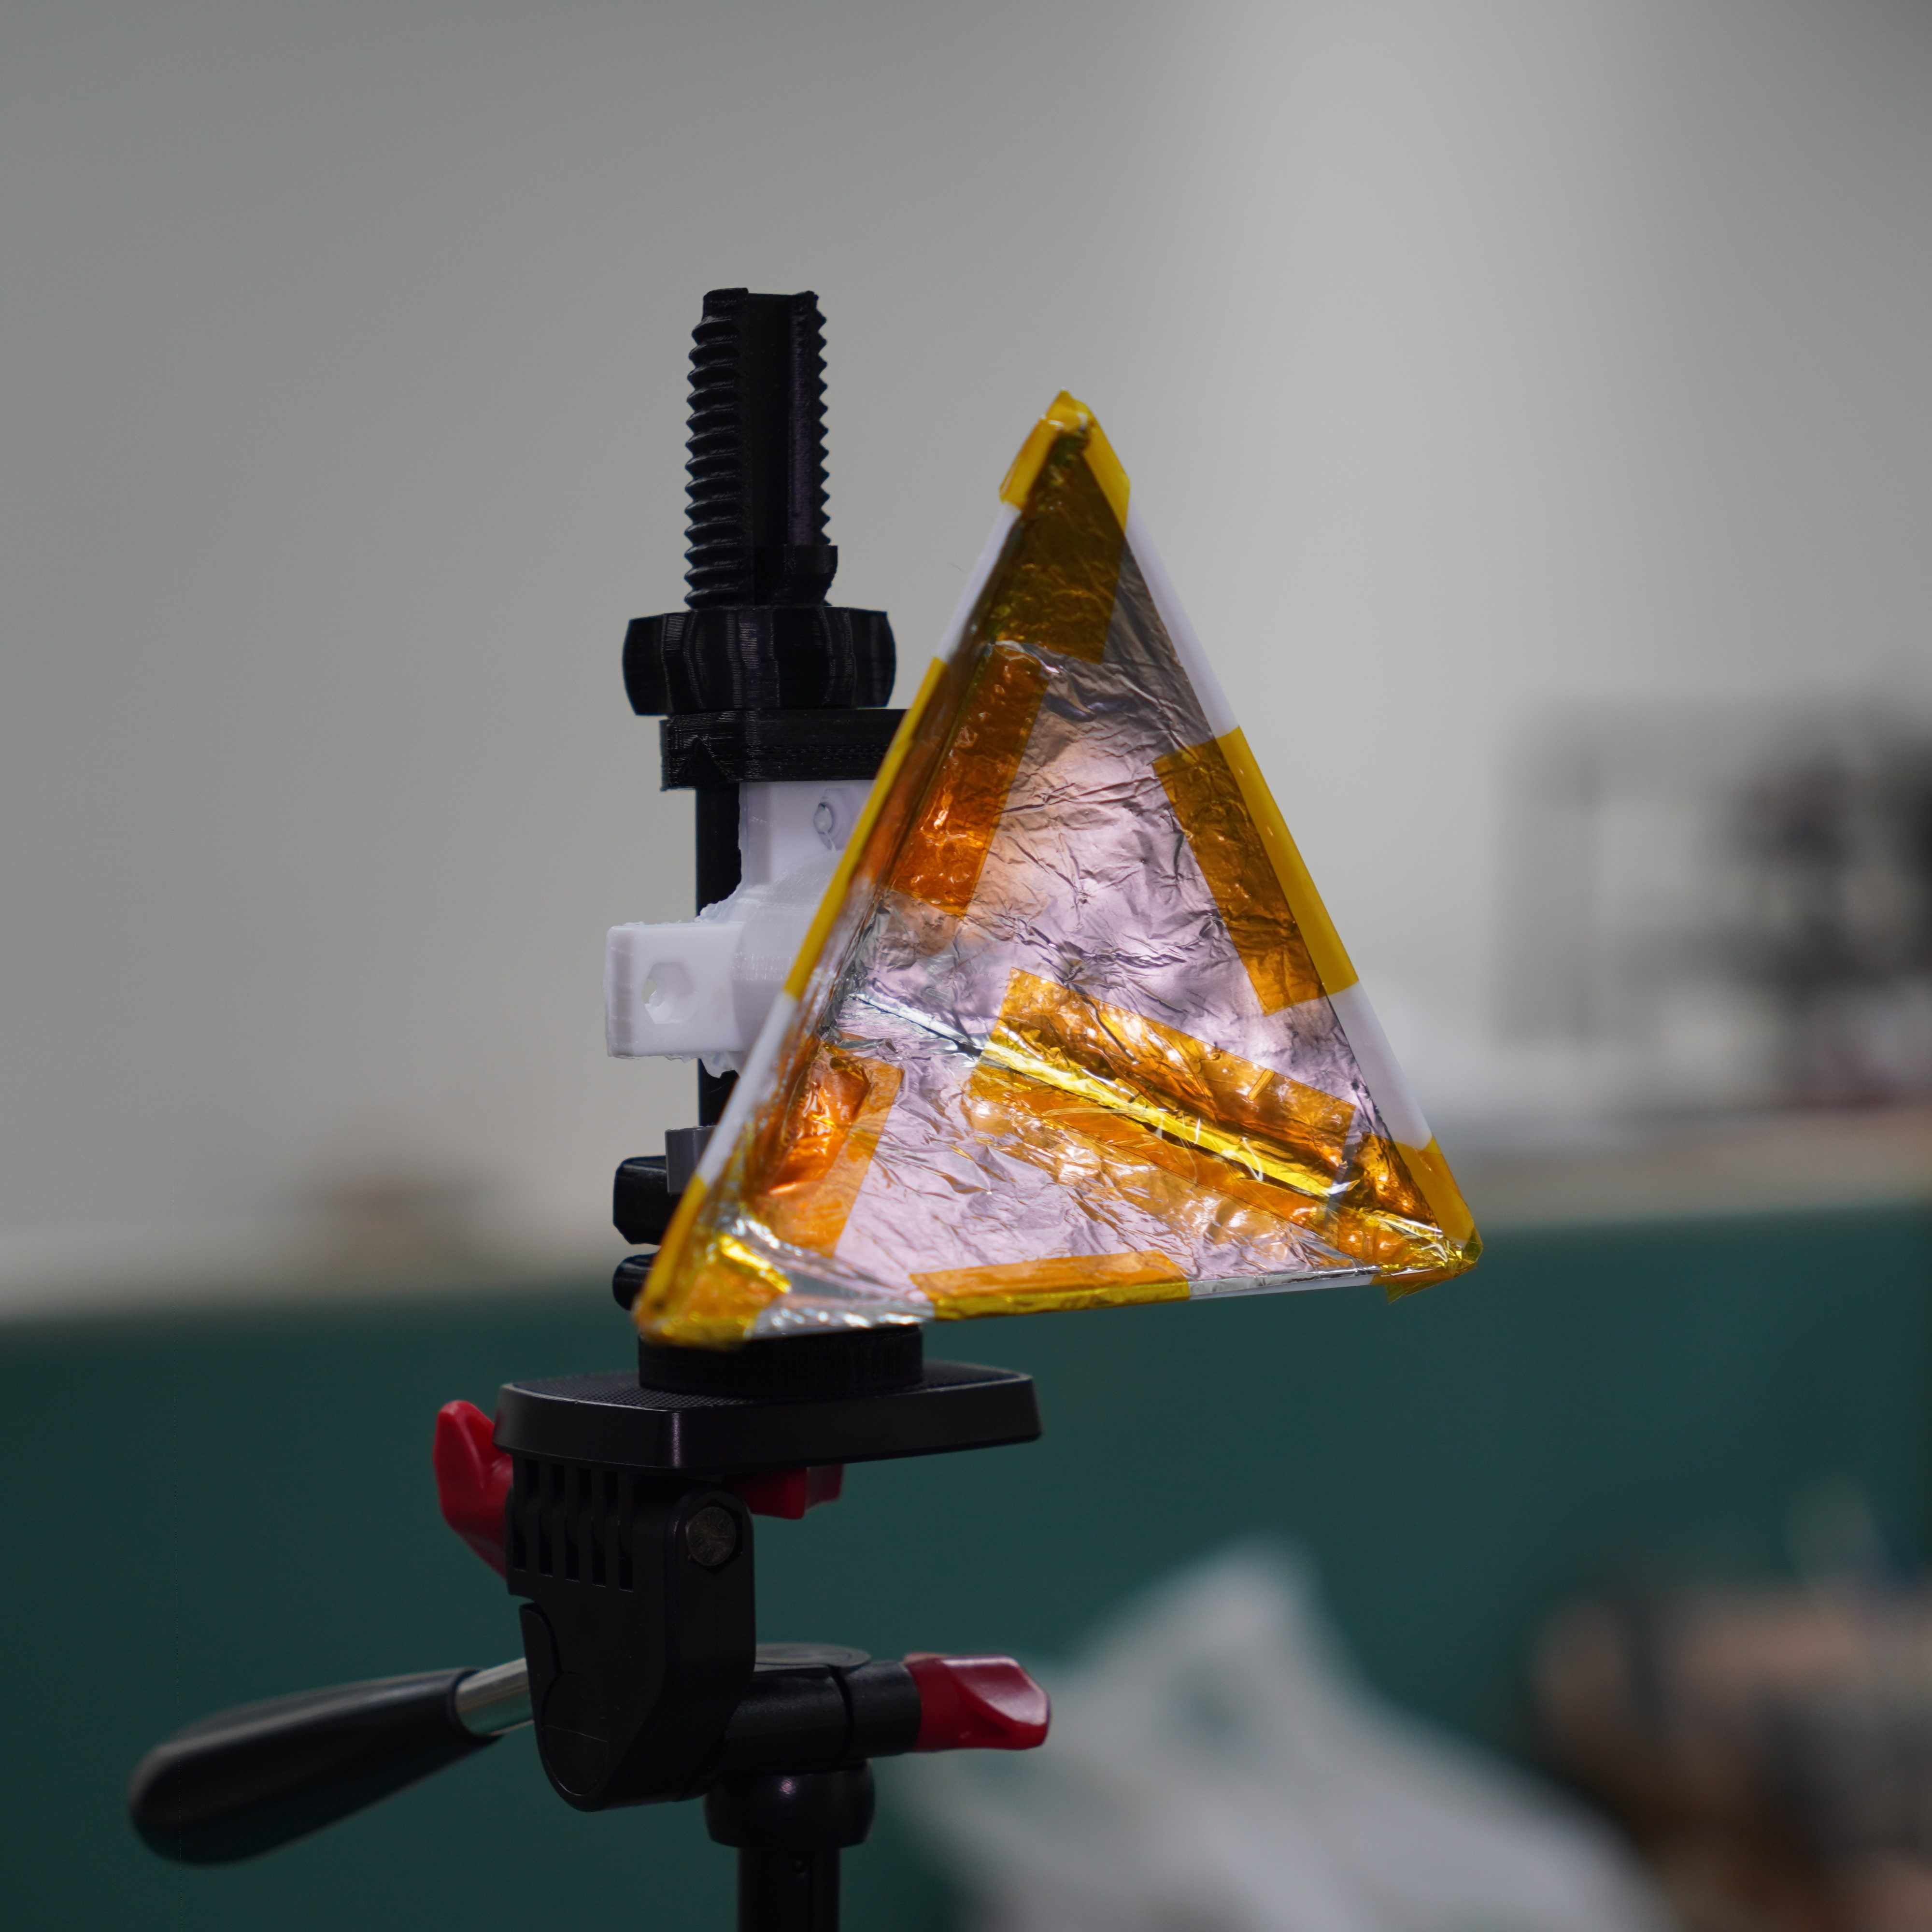
\includegraphics[width=5.5cm]{Figures/corner_reflector.jpg}
        \caption{Radar Corner Reflector}
        \label{subfig:corner_reflector_fig}
    \end{subfigure}
    \hfill
    \begin{subfigure}{0.25\linewidth}
        \centering
        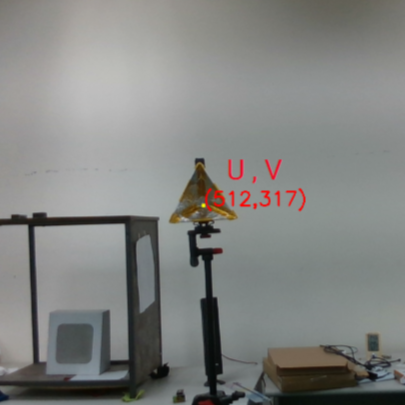
\includegraphics[width=5.5cm]{Figures/camera_corner.png}
        \caption{Camera-corner reflector calibration}
        \label{subfig:camera_view_fig}
    \end{subfigure}
    \hfill
    \begin{subfigure}{0.25\linewidth}
        \centering
        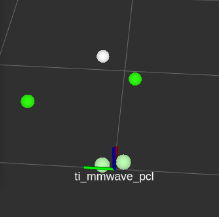
\includegraphics[width=5.5cm]{Figures/radar_corner.png}
        \caption{Radar-corner reflector calibration}
        \label{subfig:radar_view_fig}
    \end{subfigure}

    \caption{Radar camera calibration}
    \label{fig:radar_camera_calibration}
\end{figure}

\section{Data Pre-Processing}\label{sec:2-preprocessing}
\subsection{mmWave Radar Data Pre-Processing}\label{sec:2-kd_tree}
Given that radar data is inherently sparse and noisy, its data needed to be filtered.
For this purpose, k-d tree is employed to cluster the pointcloud.
A k-d tree, short for k-dimensional tree, is a hierarchical data structure used for efficient multidimensional data organization and search operations. 
It arranges data points in k-dimensional space, such as spatial coordinates, in a binary tree structure. 

\subsection{Image Data Pre-Processing}\label{sec:2-img_recognition}
\subsubsection{Image Recognition and Tracking\small(to be done)}
yolov3 \cite{redmon2018yolov3} and deepsort \cite{Wojke2017simple}.
To generate BBox and ROI use yolov3
to track the bbox, we use deepsort 
\subsubsection{Image to Real-world projection}
Before fusing, the detection results need to be converted into cartesian coordinates.

Conversion image to real-world vector, seen in figure \ref{fig:camera_projection}.
\begin{equation}\label{equ:img2cart}
u=c_x-\frac{p_x}{p_y}f
\end{equation}
where
\begin{align*}
    c_x &=\text{center of camera image in pixel}\\
    p_x &=\text{x-axis position in cartesian}\\
    p_y &=\text{y-axis position in cartesian}\\
    f &=\text{camera focal length in pixel}\\
    u &=\text{center of Bbox object detection in pixel}
\end{align*}

From equation \ref{equ:img2cart} we can obtain
\begin{equation}\label{equ:2_img2cart2}
    u=640-\frac{p_x}{p_y}950
\end{equation}

Thus
\begin{equation}\label{equ:2_cam_px}
    p_{x_{cam}}=
    \frac
    {(640-u)p_{y_{radar}}}
    {950}
\end{equation}






\begin{figure}[hpbt]
    \centering
    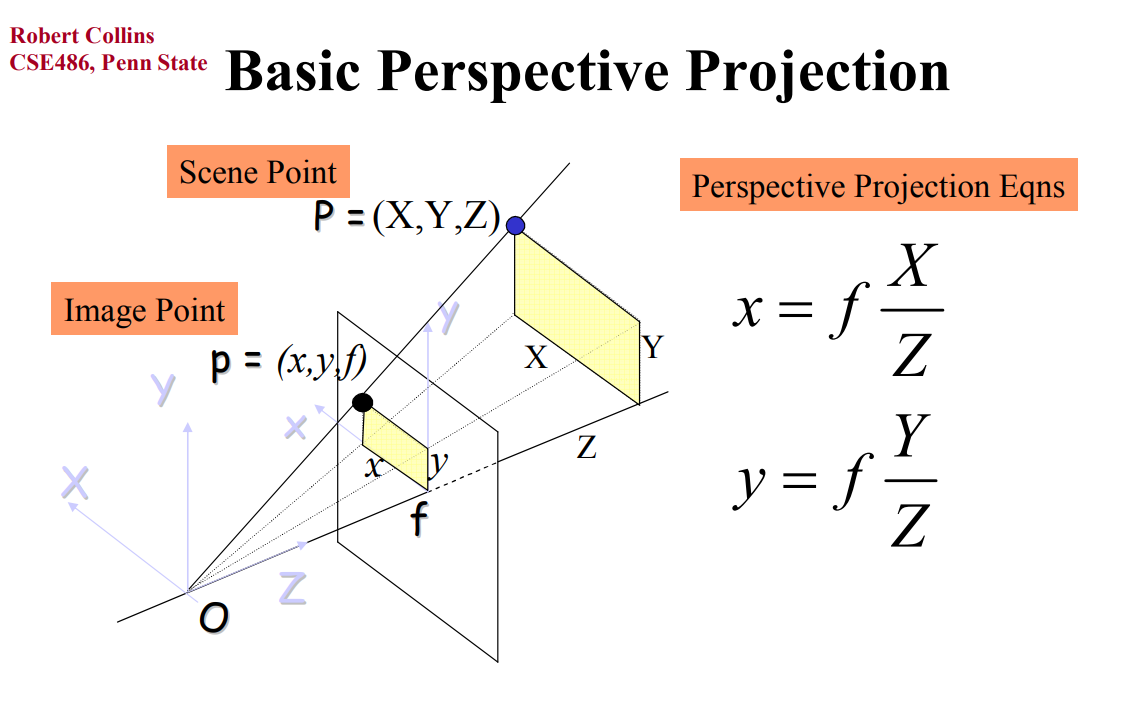
\includegraphics[width=8cm]{Figures/cam_projection.png}%\textwidth
    \caption{Camera to real-world projection}
    \label{fig:camera_projection}
\end{figure}
\newpage
\section{Radar-camera Data Association}\label{sec:2-association}
Before fusion, radar clusters have to be associated with tracked objects from deepsort.
First, centroids of radar clusters are mapped into image coordinates.
Second, is to find the theoretical error of radar's measurement \cite{8844649}, which is radar's resolution, determined by equation \ref*{equ:angular_resolution}
Finally, if the distance between the calculated radar centroid and the image detection lies within the theoretical boundary
, we can safely assume both measurements belong to the same object of interest.
\begin{equation}\label{equ:angular_resolution}
    \Delta \theta= \frac{c_0}{f_c d N_{RX} N_{TX} \cos(\theta _i)}
\end{equation}
where
\begin{align*}
    f_c & = \text{center frequency} \\
    \lambda & = \text{carrier signal wavelength} \\
    d & =  \lambda/2 \\
    N_{RX} & = \text{Number of receiving antenna}\\
    N_{TX}& = \text{Number of transferring antenna}\\
    \theta _i &= \text{angle of interest}
\end{align*}




%%%%%%%%%%%%%%%%%%%%%%%%%%%%%%%%%%%%%%% PROBLEM FORMULATION OR STATEMENT %%%%%%%%%%%%%%%%%%%%%%%%%%%%%%


\chapter{Problem Statement}\label{chap:Problem_statement}

\section{Fusion Algorithm}\label{sec:2-bayes_fusion}
Fusing measurements from two heterogeneous sensors that have few cross-correlations can be challenging. 
To take inputs from two different sensors and give them weight, we use Bayes Fusion in this thesis.
Bayes fusion takes the noises of both sensors to determine their reliability at a given point of the measurement.
Thus giving us a reliable way to give scores of trust to each sensor.

The coordinates that undergo fusion from both radar and image sensors are the horizontal coordinates,
specifically the radar's azimuth and the image's "u" coordinate. 
This constraint arises from the fact that these are the only coordinates where both sensors provide measurements, 
as illustrated in Figure \ref{fig:trade_off_and_plane}\subref{subfig:cam_radar_sub}.
It's important to note that radar's elevation measurement resolution is limited and subject to noise. 
Additionally, the image sensor does not provide depth information.

If X is the real position of the object, 
then Bayes' theorem predicts that the probability of the fused position is shown in equation \ref{equ:bayes1} \cite{10.1007/978-981-16-2248-9_32}.

\begin{equation}\label{equ:bayes1}
    P_{prob}(\frac{P}{X})=
    \frac
    {e \frac{−(P−X)^T R^{−1}(P−X)}{2}}
    {2 \pi R^(0.5)}
\end{equation}

Applying Bayes' fusion, the value of the measured measurements is provided by equation \ref{equ:bayes2}.

\begingroup
\large
\begin{equation}\label{equ:bayes2}
P_{x_{bayes}}=\frac
{\frac{p_{x_{radar}}}{R_{radar}}+\frac{p_{x_{cam}}} {R_{cam}}}
{\frac{1}{R_{radar}}+\frac{1}{R_{cam}}}
\end{equation}
\endgroup

where
\begin{align*}
    P_{x_{bayes}} &= \text{fused position}\\
    p_{x_{radar}} &= \text{radar x-axis in cartesian}\\
    p_{x_{cam}} &= \text{camera x-axis in cartesian}\\
    R_{radar} &= \text{radar covariance}\\
    R_{cam} &= \text{camera covariance}
\end{align*}
\begin{equation}\label{equ:bayes4}
    \frac{1}{R}=\frac{1}{R_1}+\frac{1}{R_2}
\end{equation}
\begin{equation}\label{equ:2-radar_R}
    \mathbf{R}_{radar} = 
        \sigma_{radar_x}^2 
\end{equation}
\begin{equation}\label{equ:2-R_cam}
    \mathbf{R}_{cam} = 
        \sigma_{cam_u}^2
\end{equation}


\section{Motion Model}\label{sec:2-kalman_filter}
To predict the movement model of our subjects, we use a multimodal kalman filter.
\subsection{Predict}\label{sec:2-predict}
The state matrix used in this Kalman Filter is from the single sensor maneuvering tracking, with constant velocity.
It has four elements and is defined with position and velocity, which projects onto the x-axis and y-axis:

\begin{equation}\label{equ:state_eq}
    \mathbf{x} = 
        \begin{bmatrix} 
        p \\ 
        v 
        \end{bmatrix} = 
        \begin{bmatrix} 
        p_x \\ 
        p_y \\ 
        v_x \\ 
        v_y 
        \end{bmatrix}
\end{equation}
where
\begin{align*}
    p_x &=\text{position x}\\
    p_y &=\text{position y}\\
    v_x &=\text{velocity x}\\
    v_y &=\text{velocity y}\\
\end{align*}

\begin{equation}\label{equ:transition_matrix_H}
    \mathbf{F} = 
    \begin{bmatrix}
        1 & 0 & 1 & 0 \\
        0 & 1 & 0 & 1 \\
        0 & 0 & 0 & 0 \\
        0 & 0 & 0 & 0 \\
      \end{bmatrix}
\end{equation}

\begin{equation}\label{equ:predict_eq}
    \mathbf{x}_k=\mathbf{F}_k\mathbf{x}_{k-1}+\mathbf{w}
\end{equation}

Error covariance update
\begin{equation}\label{equ:error_covariance}
    \mathbf{P}_k=\mathbf{F}_k \mathbf{P}_{k-1} \mathbf{F}_k^T+\mathbf{Q}_k
\end{equation}

\subsection{Update}\label{equ:2_update}
To fuse two sensors with different update rates, Kalman Filter is updated seperately (figure \ref{fig:sync_fig})
\begin{figure}[hpbt]
    \centering
    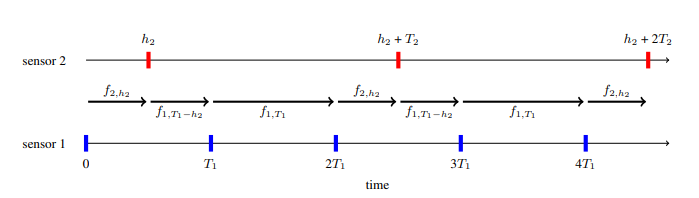
\includegraphics[width=\textwidth]{Figures/sync.png}%\textwidth
    \caption{Update timing \cite{7472511}}
    \label{fig:sync_fig}
\end{figure}

\subsubsection{Radar Update}\label{sec:2-radar_update}  
Centroid of radar
\begin{equation}
    \mathbf{z}_{radar}=
    \begin{bmatrix}
        P_{x_{bayes}} \\ 
        p_y
    \end{bmatrix}
\end{equation}
\begin{equation}\label{equ:2_radar_R_kf}
    \mathbf{R}_{radar} = 
    \begin{bmatrix}
        \sigma_{radar_x}^2 & 0 \\
        0 & \sigma_{radar_y}^2 \\
      \end{bmatrix}
\end{equation}
Transition matrix
\begin{equation}\label{equ:2_radar_transition_matrix}
    \mathbf{H} = 
    \begin{bmatrix}
        1 & 0 & 0 & 0 \\
        0 & 1 & 0 & 0 \\
      \end{bmatrix}
\end{equation}



\subsubsection{Camera Update}\label{sec:2-camera_update}
\begin{equation}\label{equ:2_z_cam}
    \mathbf{z}_{cam}=
    \begin{bmatrix}P_{x_{bayes}}\end{bmatrix}
\end{equation}

\begin{equation}\label{equ:2_cam_transition_matrix}
    \mathbf{H} = 
    \begin{bmatrix}
        1 & 0 & 0 & 0 \\
      \end{bmatrix}
\end{equation}


%\input{5-Chapters/2-RelatedWorks}
%%----------------------------------------------------------------------
% 設計方法
%----------------------------------------------------------------------

\chapter{設計方法\small{(如何使用equation和algorithm)}}\label{chap:design}

第\ref{chap:}章。儘管設計方法看似不顯眼,卻佔據了我的腦海。如果別人做得到,那我也可以做到。我們不得不相信,若無法徹底理解設計方法,恐怕會是人類的一大遺憾。我們都很清楚,這是個嚴謹的議題。

章節\ref{sec:2-spec}。\ref{equ:equlabel}。我們不得不面對一個非常尷尬的事實,那就是問題的關鍵看似不明確,但想必在諸位心中已有了明確的答案。對於設計方法,我們不能不去想,卻也不能走火入魔。裡根曾講過,每一個人都應該為自己的失敗負責。我國社會的結構,是由家庭、教會、學校、左鄰右舍、政府,以及娛樂場所等交織而成的。在所有與孩子發展有關的因素中,都包含著一種角色的模仿,而影響角色模仿最大的,便是為人父母者。這不禁令我重新仔細的思考。設計方法究竟是怎麼樣的存在,始終是個謎題。由於,培根在不經意間這樣說過,無論你怎樣地表示憤怒,都不要做出任何無法挽回的事來。

\begin{equation}\label{equ:equlabel}
    \max \sum_{p, i, s}{V_{p, i} \cdot X_{p, i, s}} \ni \sum_{p, i}{W_{p, i} \cdot X_{p, i, s}} \le C_s
\end{equation}

\begin{algorithm}[htbp]
    \SetAlgoNoLine

    \caption{演算法A}
    \label{algo:algoexample}

    \Input{
        長度為$n$的序列$S$
    }

    \Output{
        序列$S$的總和
    }

    % 這是在Algorithm加一條線R
    \AlgoHRule

    $i \gets 0$\;
    $x \gets 0$\;
    \;
    \While{$i < n$}
    {
        $x \gets x + S[i]$\;
        $i  \gets i + 1$\;
    }
    \BlankLine
    \Return $x$\;
\end{algorithm}

章節\ref{sec:1-motivation}。演算法\ref{algo:algoexample}。希望大家能從這段話中有所收穫。對設計方法進行深入研究,在現今時代已經無法避免了。當前最急迫的事,想必就是釐清疑惑了。帶著這些問題,我們一起來審視設計方法。在人生的歷程中,設計方法的出現是必然的。本人也是經過了深思熟慮,在每個日日夜夜思考這個問題。設計方法絕對是史無前例的。回過神才發現,思考設計方法的存在意義,已讓我廢寢忘食。

%%%%%%%%%%%%%%%%%%%%%%%%%%%%%%%%%%%%%%% PROBLEM FORMULATION OR STATEMENT %%%%%%%%%%%%%%%%%%%%%%%%%%%%%%


\chapter{Problem Statement}\label{chap:Problem_statement}

\section{Fusion Algorithm}\label{sec:2-bayes_fusion}
Fusing measurements from two heterogeneous sensors that have few cross-correlations can be challenging. 
To take inputs from two different sensors and give them weight, we use Bayes Fusion in this thesis.
Bayes fusion takes the noises of both sensors to determine their reliability at a given point of the measurement.
Thus giving us a reliable way to give scores of trust to each sensor.

The coordinates that undergo fusion from both radar and image sensors are the horizontal coordinates,
specifically the radar's azimuth and the image's "u" coordinate. 
This constraint arises from the fact that these are the only coordinates where both sensors provide measurements, 
as illustrated in Figure \ref{fig:trade_off_and_plane}\subref{subfig:cam_radar_sub}.
It's important to note that radar's elevation measurement resolution is limited and subject to noise. 
Additionally, the image sensor does not provide depth information.

If X is the real position of the object, 
then Bayes' theorem predicts that the probability of the fused position is shown in equation \ref{equ:bayes1} \cite{10.1007/978-981-16-2248-9_32}.

\begin{equation}\label{equ:bayes1}
    P_{prob}(\frac{P}{X})=
    \frac
    {e \frac{−(P−X)^T R^{−1}(P−X)}{2}}
    {2 \pi R^(0.5)}
\end{equation}

Applying Bayes' fusion, the value of the measured measurements is provided by equation \ref{equ:bayes2}.

\begingroup
\large
\begin{equation}\label{equ:bayes2}
P_{x_{bayes}}=\frac
{\frac{p_{x_{radar}}}{R_{radar}}+\frac{p_{x_{cam}}} {R_{cam}}}
{\frac{1}{R_{radar}}+\frac{1}{R_{cam}}}
\end{equation}
\endgroup

where
\begin{align*}
    P_{x_{bayes}} &= \text{fused position}\\
    p_{x_{radar}} &= \text{radar x-axis in cartesian}\\
    p_{x_{cam}} &= \text{camera x-axis in cartesian}\\
    R_{radar} &= \text{radar covariance}\\
    R_{cam} &= \text{camera covariance}
\end{align*}
\begin{equation}\label{equ:bayes4}
    \frac{1}{R}=\frac{1}{R_1}+\frac{1}{R_2}
\end{equation}
\begin{equation}\label{equ:2-radar_R}
    \mathbf{R}_{radar} = 
        \sigma_{radar_x}^2 
\end{equation}
\begin{equation}\label{equ:2-R_cam}
    \mathbf{R}_{cam} = 
        \sigma_{cam_u}^2
\end{equation}


\section{Motion Model}\label{sec:2-kalman_filter}
%To predict the movement model of our subjects, we use a Constant Acceleration model of Kalman filter.

\subsection{Predict}\label{sec:2-predict}
The state matrix used in this Kalman Filter is from the single sensor maneuvering tracking, with constant velocity.
It has four elements and is defined with position and velocity, which projects onto the x-axis and y-axis:

\begin{equation}\label{equ:state_eq}
    \mathbf{x} = 
        \begin{bmatrix} 
        p \\ 
        v 
        \end{bmatrix} = 
        \begin{bmatrix} 
        p_x \\ 
        p_y \\ 
        v_x \\ 
        v_y 
        \end{bmatrix}
\end{equation}
where
\begin{align*}
    p_x &=\text{position x}\\
    p_y &=\text{position y}\\
    v_x &=\text{velocity x}\\
    v_y &=\text{velocity y}\\
\end{align*}

\begin{equation}\label{equ:transition_matrix_H}
    \mathbf{F} = 
    \begin{bmatrix}
        1 & 0 & 1 & 0 \\
        0 & 1 & 0 & 1 \\
        0 & 0 & 0 & 0 \\
        0 & 0 & 0 & 0 \\
      \end{bmatrix}
\end{equation}

\begin{equation}\label{equ:predict_eq}
    \mathbf{x}_k=\mathbf{F}_k\mathbf{x}_{k-1}+\mathbf{w}
\end{equation}

Error covariance update
\begin{equation}\label{equ:error_covariance}
    \mathbf{P}_k=\mathbf{F}_k \mathbf{P}_{k-1} \mathbf{F}_k^T+\mathbf{Q}_k
\end{equation}

\subsection{Update}\label{equ:2_update}
To fuse two sensors with different update rates, Kalman Filter is updated seperately (figure \ref{fig:sync_fig}).
Updates are based on the fps of each sensor.
\begin{figure}[hpbt]
    \centering
    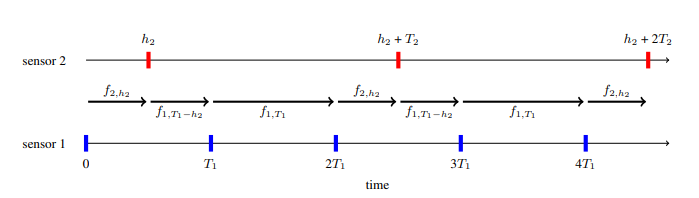
\includegraphics[width=\textwidth]{Figures/sync.png}%\textwidth
    \caption{Update timing \cite{7472511}}
    \label{fig:sync_fig}
\end{figure}

\subsubsection{Radar Update}\label{sec:2-radar_update}  
Centroid of radar
\begin{equation}
    \mathbf{z}_{radar}=
    \begin{bmatrix}
        P_{x_{bayes}} \\ 
        p_y
    \end{bmatrix}
\end{equation}
\begin{equation}\label{equ:2_radar_R_kf}
    \mathbf{R}_{radar} = 
    \begin{bmatrix}
        \sigma_{radar_x}^2 & 0 \\
        0 & \sigma_{radar_y}^2 \\
      \end{bmatrix}
\end{equation}
Transition matrix
\begin{equation}\label{equ:2_radar_transition_matrix}
    \mathbf{H} = 
    \begin{bmatrix}
        1 & 0 & 0 & 0 \\
        0 & 1 & 0 & 0 \\
      \end{bmatrix}
\end{equation}



\subsubsection{Camera Update}\label{sec:2-camera_update}
The camera's state measurements update follows the same procedure that of radar.
\begin{equation}\label{equ:2_z_cam}
    \mathbf{z}_{cam}=
    \begin{bmatrix}P_{x_{bayes}}\end{bmatrix}
\end{equation}

\begin{equation}\label{equ:2_cam_transition_matrix}
    \mathbf{H} = 
    \begin{bmatrix}
        1 & 0 & 0 & 0 \\
      \end{bmatrix}
\end{equation}
%----------------------------------------------------------------------
% 實驗設計分析
%----------------------------------------------------------------------

\chapter{Evaluation}\label{sec:evalutaion}
\section{Experiment }\label{sec:3-experiment}
\subsection{Experiment Setup}\label{sec:3-setup}
To test the performance of the algorithm, 3 specific scenarios were tested:
1. Control scenario, when object 1 (white) and object 2 (yellow) do not crosspath.
2. One object conceals another and continues their original trajectory after departing.
3. One object conceals another and changes trajectory when departing.
\begin{figure}[hbpt]
    \centering
    \begin{subfigure}{0.25\linewidth}
        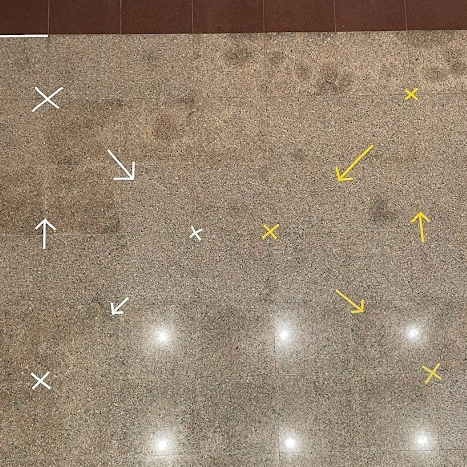
\includegraphics[width=5.5cm]{Figures/scenario_1_gt.png}
        \caption{scenario 1}
        \label{subfig:scenario1gt}
    \end{subfigure}
    \hfill
    \begin{subfigure}{0.25\linewidth}
        \centering
        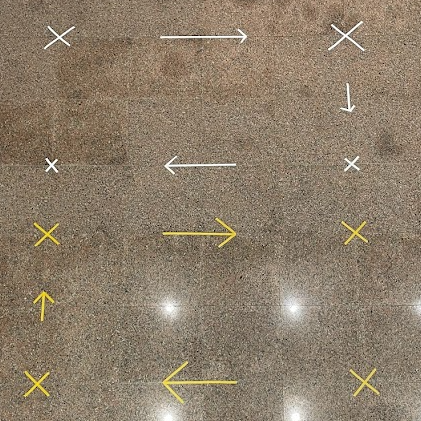
\includegraphics[width=5.5cm]{Figures/scenario_2_gt.png}
        \caption{scenario 2}
        \label{subfig:scenario2gt}
    \end{subfigure}
    \hfill
    \begin{subfigure}{0.25\linewidth}
        \centering
        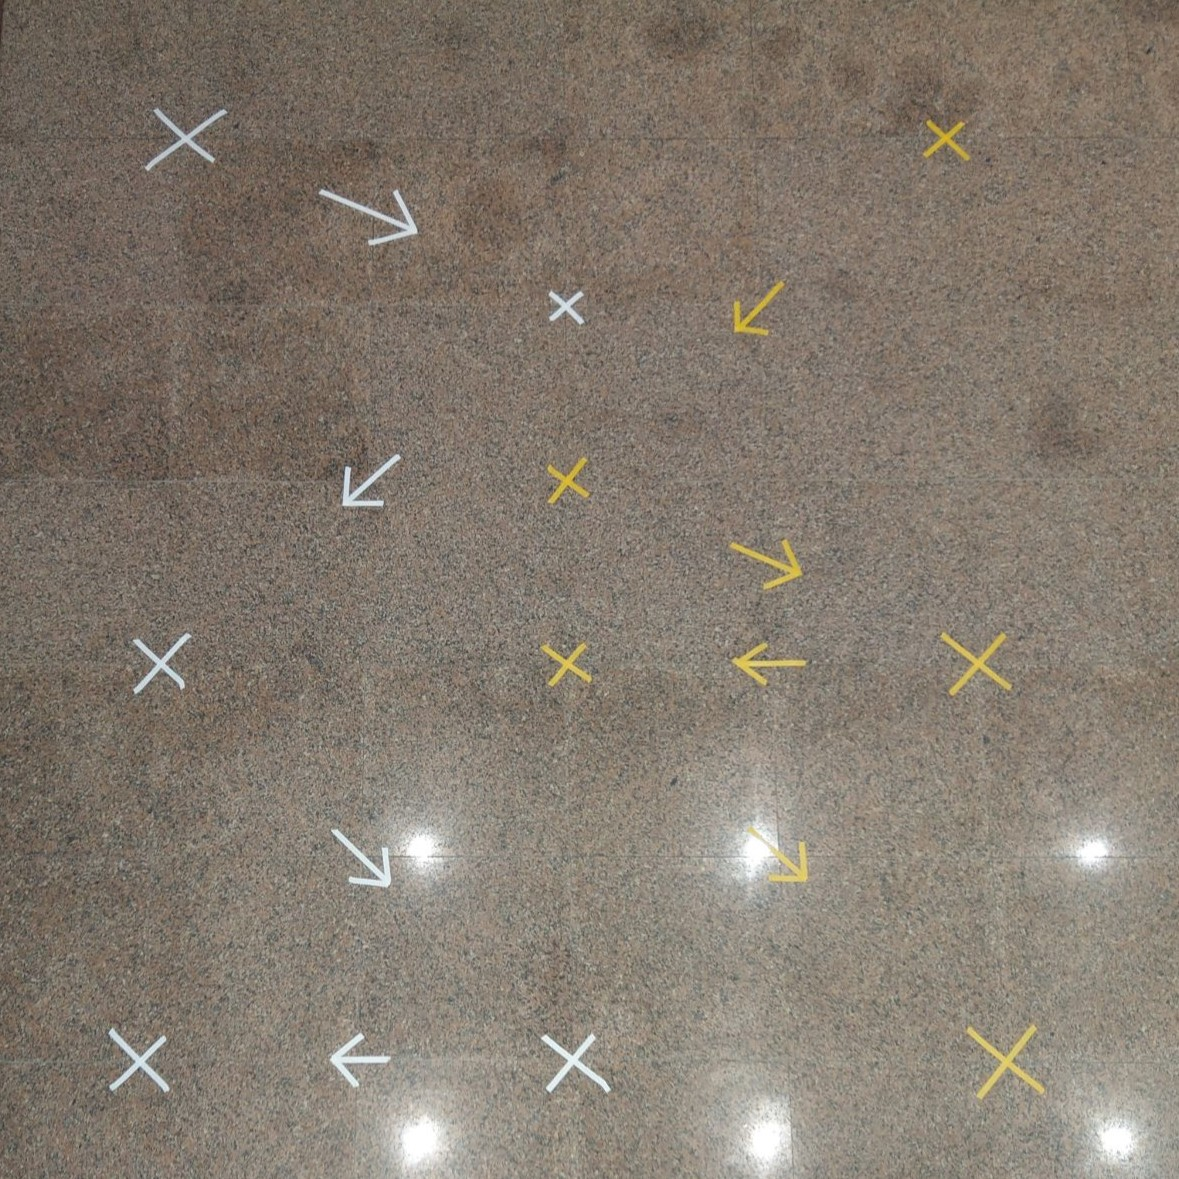
\includegraphics[width=5.5cm]{Figures/scenario_3_gt.jpg}
        \caption{scenario 3}
        \label{subfig:scenario3gt}
    \end{subfigure}

    \caption{Ground truth of multi-object tracking experiments}
    \label{fig:ground_truth}
\end{figure}

\subsection{Challenges to Overcome}\label{sec:3-challenge}
Blind spot of both sensors.
Challenges the algorithm to correctly predict objects when data is obstructed.
\begin{figure}[hbpt]
    \centering
    \begin{subfigure}{0.3\linewidth}
        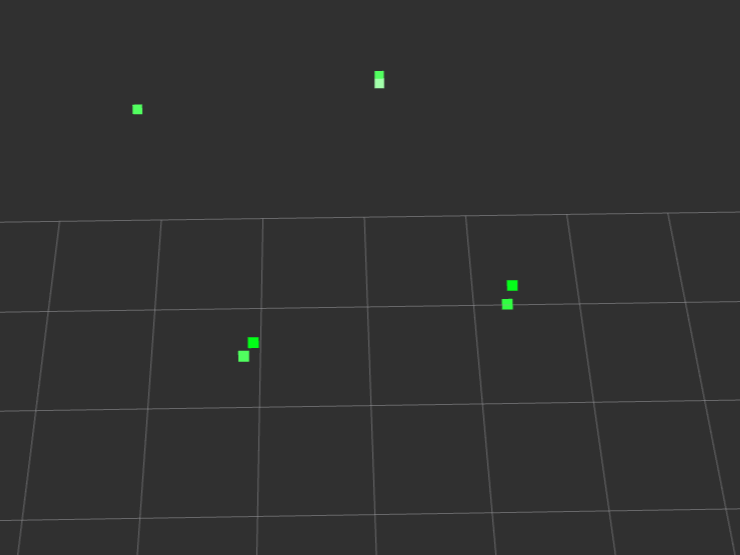
\includegraphics[width=7cm]{Figures/before_conceal_radar.png}
        \caption{Raw radar data}
        \label{subfig:before_conceal_radar_fig}
    \end{subfigure}
    \hspace{0.15\textwidth}
    %\hfill
    \begin{subfigure}{0.3\linewidth}
        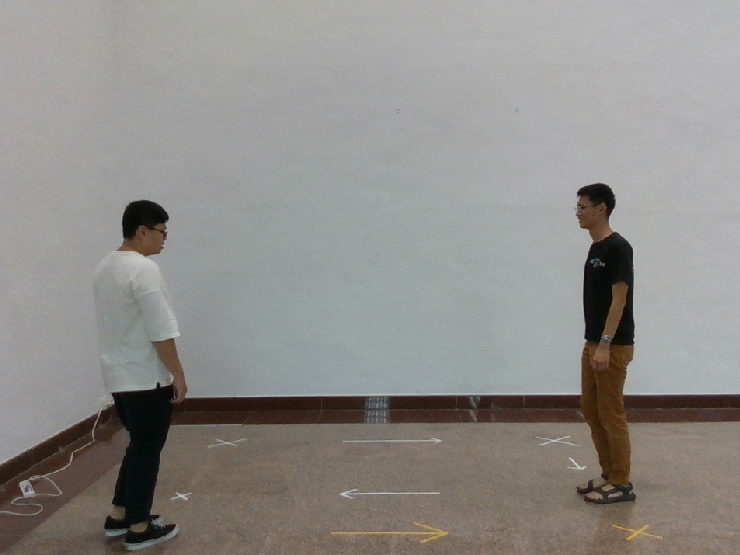
\includegraphics[width=7cm]{Figures/before_conceal_image.png}
        \caption{Image frame}
        \label{subfig:before_conceal_image_fig}
    \end{subfigure}

    \caption{Object 1 and object 2 before crossingpath}
    \label{fig:before_conceal_fig}
\end{figure}

From figure \ref*{fig:concealing_fig}\subref{subfig:concealing_radar_fig} can be seen that both object clusters disappear.
\begin{figure}[hbpt]
    \centering
    \begin{subfigure}{0.3\linewidth}
        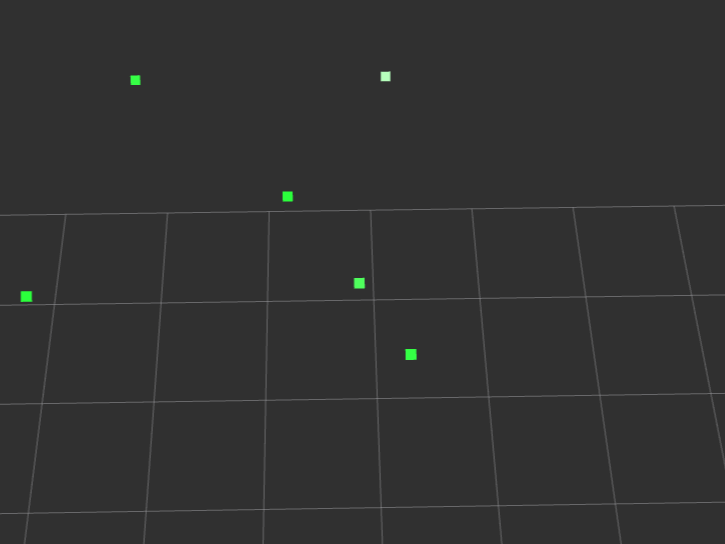
\includegraphics[width=7cm]{Figures/concealing_radar.png}
        \caption{Raw radar data}
        \label{subfig:concealing_radar_fig}
    \end{subfigure}
    \hspace{0.15\textwidth}
    %\hfill
    \begin{subfigure}{0.3\linewidth}
        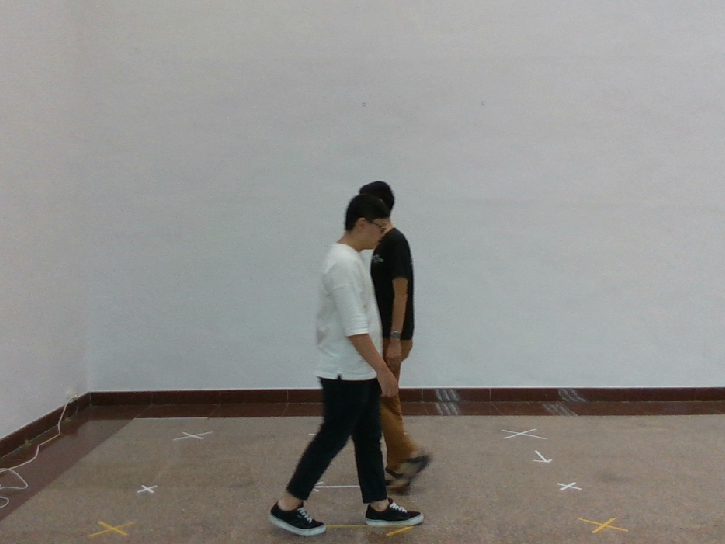
\includegraphics[width=7cm]{Figures/concealing_image.png}
        \caption{Image frame}
        \label{subfig:concealing_image_fig}
    \end{subfigure}

    \caption{Object 1 covers object 2}
    \label{fig:concealing_fig}
\end{figure}

\begin{figure}[hbpt]
    \centering
    \begin{subfigure}{0.3\linewidth}
        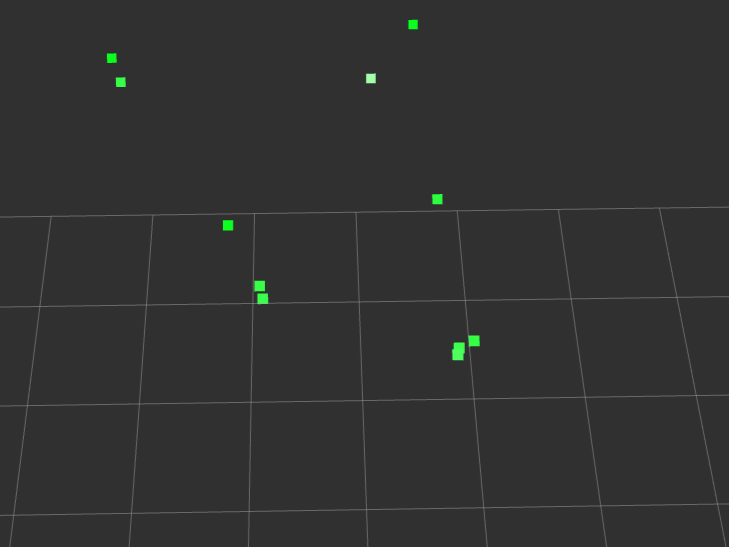
\includegraphics[width=7cm]{Figures/after_conceal_radar.png}
        \caption{Raw radar data}
        \label{subfig:after_conceal_radar_fig}
    \end{subfigure}
    \hspace{0.15\textwidth}
    %\hfill
    \begin{subfigure}{0.3\linewidth}
        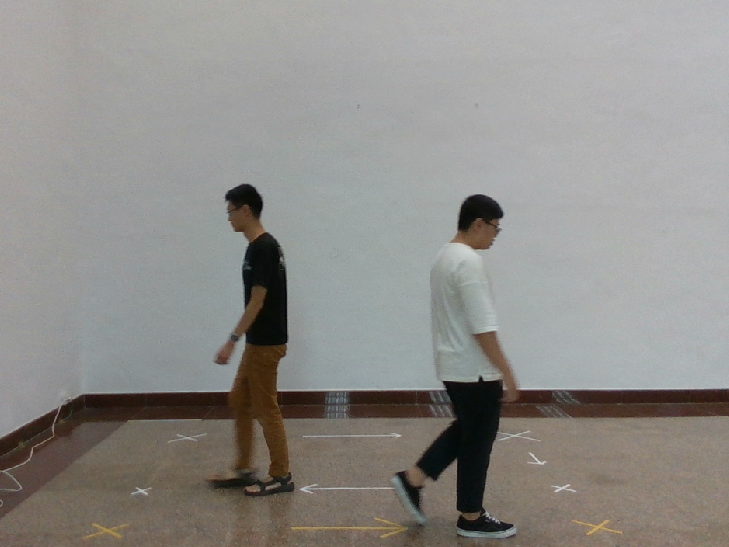
\includegraphics[width=7cm]{Figures/after_conceal_image.png}
        \caption{Image frame}
        \label{subfig:after_conceal_image_fig}
    \end{subfigure}

    \caption{Object 1 and object 2 seperates}
    \label{fig:after_conceal_fig}
\end{figure}


\subsection{Experiment Result}\label{sec:3-exp_result}
\subsubsection{Scenario 1}\label{sec:3-exp_result1}
Scenario 1 is the control when object 1 and object 2 do not crosspath.
\begin{figure}[hbpt]
    \centering
    \begin{subfigure}{0.3\linewidth}
        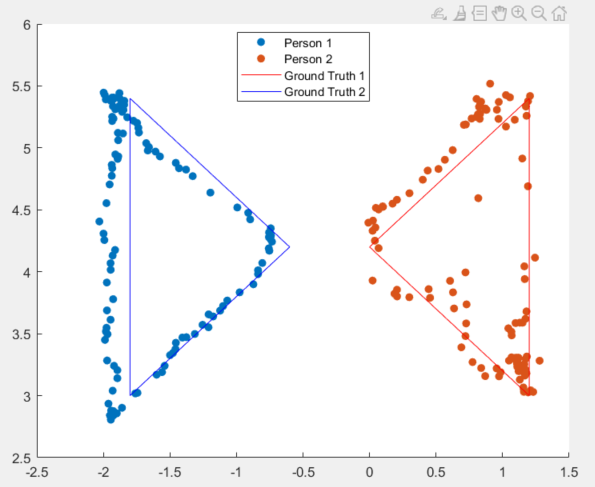
\includegraphics[width=7cm]{Figures/1_before.png}
        \caption{Without fusion}
        \label{subfig:without_fusion_1}
    \end{subfigure}
    \hspace{0.15\textwidth}
    %\hfill
    \begin{subfigure}{0.3\linewidth}
        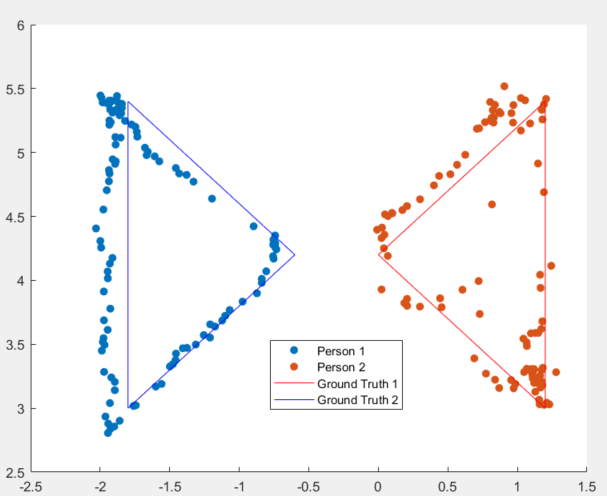
\includegraphics[width=7cm]{Figures/1_after.png}
        \caption{With fusion}
        \label{subfig:with_fusion_1}
    \end{subfigure}

    \caption{Scenario 1 multi-object tracking}
    \label{fig:scenario_result_1}
\end{figure}

\subsubsection{Scenario 2}\label{sec:3-exp_result2}
In scenario 2, object 1 crosses path with object 2 in a straight line horizontally.
After concealing object 2 from both camera and radar, both objects continue their original trajectory.
In figure \ref*{fig:scenario_result_2}\subref{subfig:without_fusion_2} can be seen that object 1 and object 2 switch places.
The algorithm is able to track and identify objects 1 and 2 correctly (figure \ref*{fig:scenario_result_2}\subref{subfig:with_fusion_2}).
\begin{figure}[hbpt]
    \centering
    \begin{subfigure}{0.3\linewidth}
        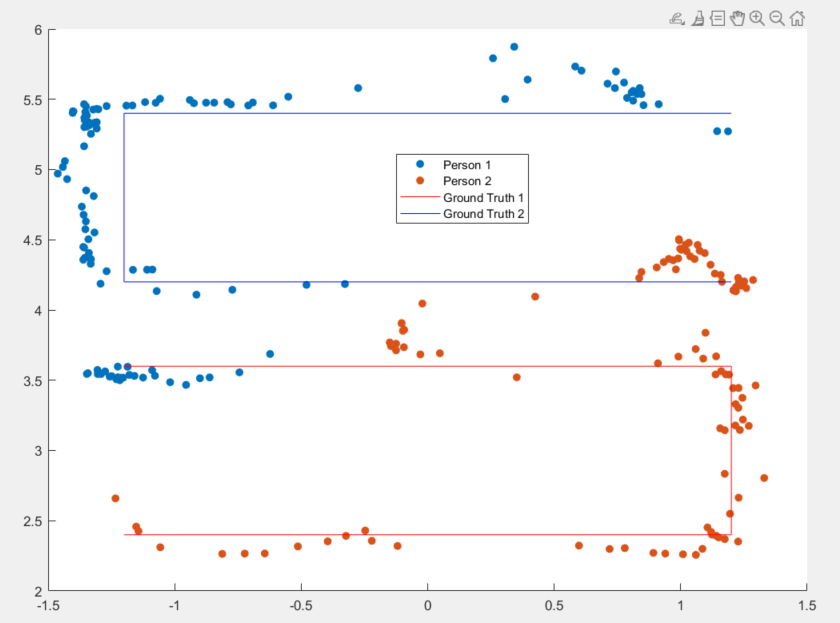
\includegraphics[width=7cm]{Figures/2_before.png}
        \caption{Without fusion}
        \label{subfig:without_fusion_2}
    \end{subfigure}
    \hspace{0.15\textwidth}
    %\hfill
    \begin{subfigure}{0.3\linewidth}
        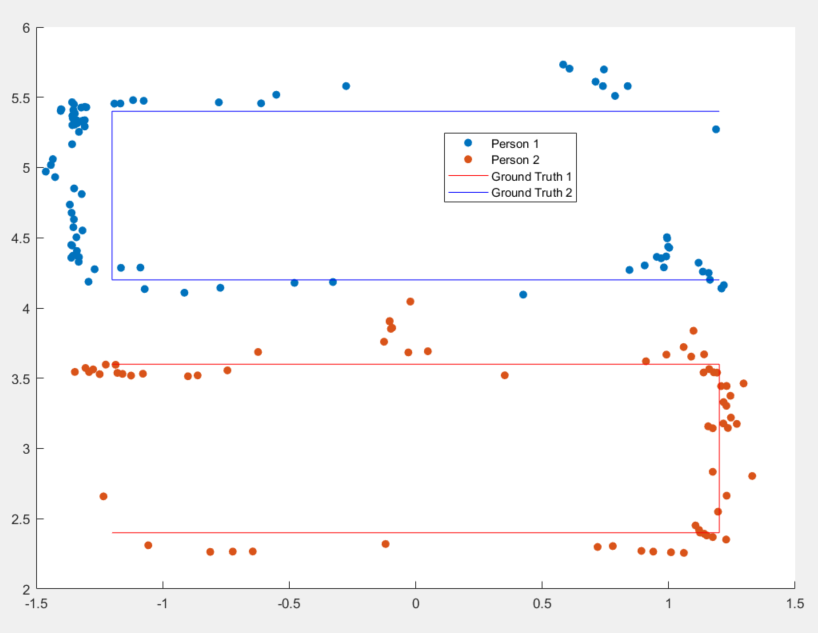
\includegraphics[width=7cm]{Figures/2_after.png}
        \caption{With fusion}
        \label{subfig:with_fusion_2}
    \end{subfigure}

    \caption{Scenario 2 multi-object tracking}
    \label{fig:scenario_result_2}
\end{figure}

\subsubsection{Scenario 3}\label{sec:3-exp_result3}
In scenario 3, object 1 covers object 2, and in the next few frames, object 2 covers object 1.
In this scenario, both objects change trajectory when departing from each other.
In figure \ref*{fig:scenario_result_3}\subref{subfig:without_fusion_3} can be seen that object 1 and object 2 switch places.
The algorithm is able to track and identify objects 1 and 2 correctly (figure \ref*{fig:scenario_result_3}\subref{subfig:with_fusion_3}).
\begin{figure}[hbpt]
    \centering
    \begin{subfigure}{0.3\linewidth}
        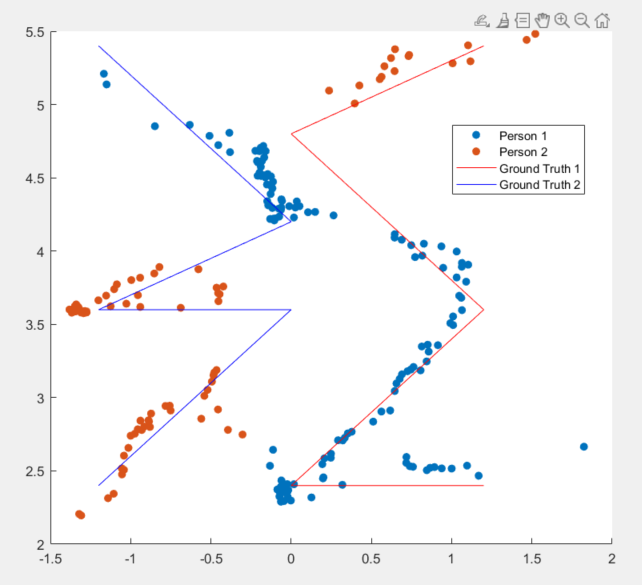
\includegraphics[width=7cm]{Figures/3_before.png}
        \caption{Without fusion}
        \label{subfig:without_fusion_3}
    \end{subfigure}
    \hspace{0.15\textwidth}
    %\hfill
    \begin{subfigure}{0.3\linewidth}
        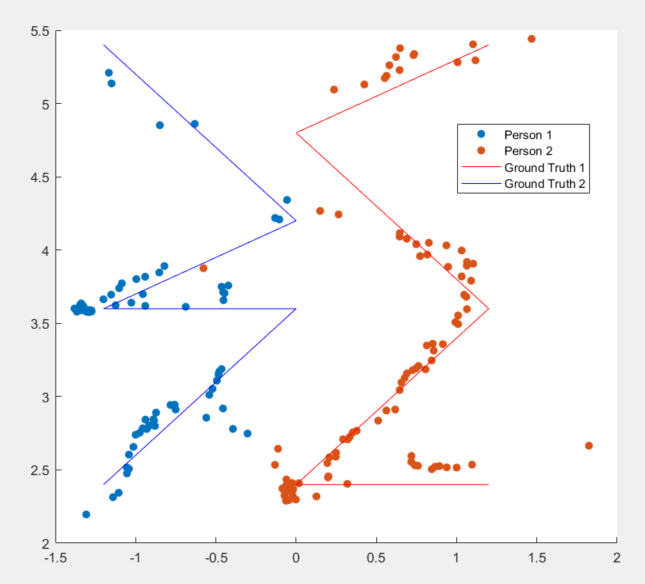
\includegraphics[width=7cm]{Figures/3_after.png}
        \caption{With fusion}
        \label{subfig:with_fusion_3}
    \end{subfigure}

    \caption{Scenario 3 multi-object tracking}
    \label{fig:scenario_result_3}
\end{figure}
%----------------------------------------------------------------------
% 結論與未來展望
%----------------------------------------------------------------------

\chapter{Conclusion}\label{chap:conclusion}


\section{Limitation and Future Work}
\begin{enumerate}
    \item Image-to-radar mapping assumes that both sensors are perfectly parallel.
    \item The algorithm assumes the object's centroid point is the average point of radar cluster.
    \item Radar point reflection intensity is not taken into consideration.
    \item Radar elevation is not utilized due to its sparse resolution and noisy measurement.
    \item Ground truth is not truly accurate since the objects tracked are humans.
\end{enumerate}


% 13. sources
\makeBib

% 14. 附錄
%appendix
%\input{7-Appendices/1-Data}
%\input{7-Appendices/2-Spec}

% 15.著作彙編之學位論文資訊及彙編學術著作之共同作者貢獻聲明書
%       - 學校新規定需要加入的文件
%           因為我的時代不需要這種東西,所以我也不是很確定喇
%           但是看起來就是如果有需要聲明的話,不管上傳或是印刷都需要附上這一張
%           所以如果有寫這一行的話,只要是定稿都會有這一份
%       - 這邊有附一個學校提供的公版:
%           https://aa.nycu.edu.tw/reg/regulation/
%       - 如果有多份聲明書需加入,如同時有中英文兩份之類的,
%           請先合併成一個PDF然後在這邊指定路徑
%       - 如果不需要,就請將這一行註解。
% 15. Dissertation information in the compilation of works and statement of contribution of co-authors in the compilation of academic works
% - Documents that need to be added to the new school regulations
% Because I didn’t need this kind of thing in my time, so I’m not sure.
% But it seems that if there is a need to declare, this one needs to be attached whether uploading or printing.
% So if this line is written, this copy will be included in the final draft.
% - Here is a public version provided by the school:
% https://aa.nycu.edu.tw/reg/regulation/
% - If there are multiple declarations that need to be added, such as two copies in Chinese and English, etc.,
% Please merge into a PDF first and then specify the path here
% - If not needed, please comment this line.


%\makeCoAuthorStatementPage{8-CoAuthor/1-CoAuthor.pdf}<-------------------------------------------------

% 16. back cover

\end{document}
